\section{Zero sets of the weakly convex smoothed duality gap}
\label{sec:safe-sdg}

Eliminating the dual comparison variable reveals two nonnegative defects.
Their decomposition identifies the exact SDG zero set through the
level-proximal subdifferential; above the uniform weak-convexity threshold it
reduces to KKT equivalence and quantitative residual bounds.

\subsection{Proximal decomposition of the SDG}

The dual comparison variable in \cref{eq:sdg-definition} can be eliminated
exactly.  Let \(r(x):=Ax-b\).  Completing the square gives the unique
maximizer
\begin{equation}
  v_{\beta_y}(x,y)
  =
  y+\beta_y^{-1}r(x)
  \label{eq:dual-comparison-maximizer}
\end{equation}
and the value
\[
  \sup_v\left\{\ip{v}{r(x)}
    -\frac{\beta_y}{2}\norm{v-y}^2\right\}
  =\ip{y}{r(x)}+\frac{1}{2\beta_y}\norm{r(x)}^2.
\]
Consequently
\begin{equation}
  \G_{\beta_x,\beta_y}(x,y)
  =
  \Lagr(x,y)
  -\inf_u\left\{\Lagr(u,y)
       +\frac{\beta_x}{2}\norm{u-x}^2\right\}
  +\frac{1}{2\beta_y}\norm{Ax-b}^2.
  \label{eq:sdg-decomposition}
\end{equation}
This formula separates a self-centered proximal defect, which measures whether
\(x\) is a global minimizer of a quadratically regularized Lagrangian, from an
explicit squared feasibility defect.  It is valid as an extended-valued
identity: if the primal infimum is \(-\infty\), then the proximal defect and
the SDG are \(+\infty\).  The extended-valued formulation therefore precedes
any attainment or uniqueness requirement; those properties enter in the
safe regime below.
Accordingly, throughout \cref{sec:safe-sdg,sec:thresholds}, the SDG is
understood on \(\dom f\times\R^m\) as a function with values in
\([0,+\infty]\).

The decomposition also fixes an important sign convention.  A larger
\(\beta_x\) means stronger proximal curvature, whereas a larger step
\(\lambda=1/\beta_x\) means weaker curvature.

For later reference, introduce the value function
\begin{equation}
  m_{\beta_x}(x,y)
  :=
  \inf_u\left\{
    \Lagr(u,y)+\frac{\beta_x}{2}\norm{u-x}^2
  \right\}.
  \label{eq:primal-comparison-value}
\end{equation}
Then the SDG is the sum of the two nonnegative quantities
\begin{equation}
  \G_{\beta_x,\beta_y}(x,y)
  =
  \underbrace{\Lagr(x,y)-m_{\beta_x}(x,y)}
              _{\text{global self-centered proximal defect}}
  +
  \underbrace{\frac{1}{2\beta_y}\norm{r(x)}^2}
              _{\text{feasibility defect}}.
  \label{eq:sdg-two-defects}
\end{equation}
The first defect uses the global value \(m_{\beta_x}\).  An inner routine
that returns only a local model value evaluates a different numerical
quantity whose zero set may differ from that characterized below.
\Cref{fig:sdg-decomposition-schematic} illustrates the two comparison
problems and their contributions to \cref{eq:sdg-two-defects}.

\begin{figure}[htbp]
  \centering
  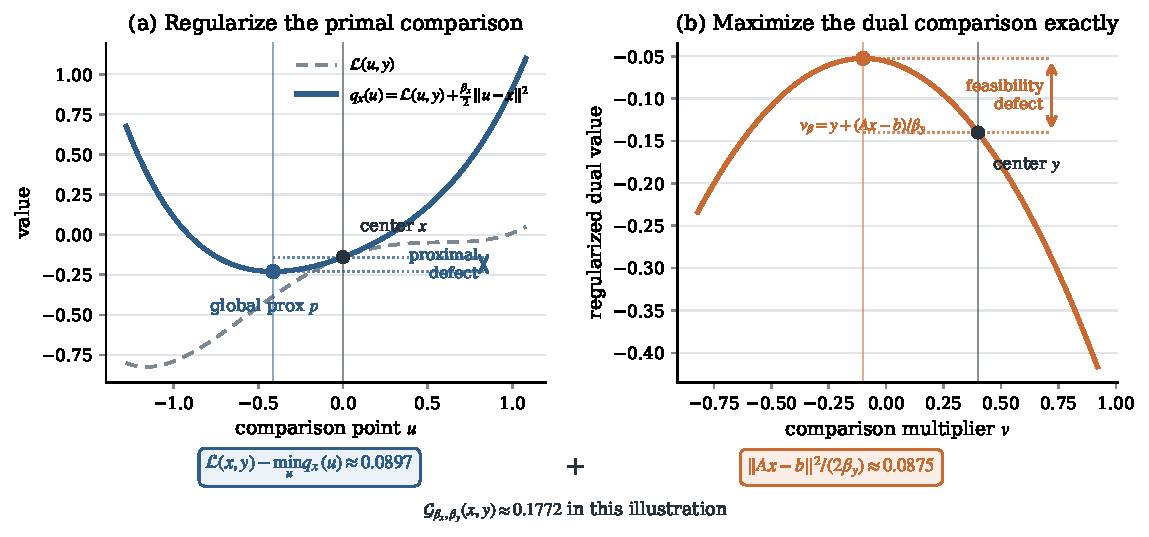
\includegraphics[width=0.98\textwidth]{figures/sdg_decomposition_schematic.pdf}
  \caption{Decomposition of a self-centered SDG evaluation.
  For \(f(u)=u^4/4-u^2/2\), \(A=1\), \(b=0.35\), \(x=0\), \(y=0.4\), and
  \((\rho,\beta_x,\beta_y)=(1,1.8,0.7)\), the global proximal decrease in
  (a) and the explicit feasibility defect in (b) sum to
  \(\G_{\beta_x,\beta_y}(x,y)\approx0.1772\).}
  \label{fig:sdg-decomposition-schematic}
\end{figure}

\begin{theorem}[Exact SDG zero set at arbitrary curvature]
  \label{thm:arbitrary-beta}
  Let \(f\) be proper and lower semicontinuous.  Fix
  \((x,y)\in\operatorname{dom}f\times\R^m\) and
  \(\beta_x,\beta_y>0\).  Interpret the SDG as an extended-valued quantity
  through the global supremum in \cref{eq:sdg-definition}.  Then
  \(\G_{\beta_x,\beta_y}(x,y)\ge0\), and
  \begin{equation}
    \G_{\beta_x,\beta_y}(x,y)=0
    \quad\Longleftrightarrow\quad
    Ax=b
    \quad\text{and}\quad
    -A^\top y\in\partial_{\mathrm p}^{\beta_x}f(x).
    \label{eq:sdg-level-prox-zero}
  \end{equation}
  In particular, every zero of the SDG is a KKT pair.
\end{theorem}

\begin{proof}
  In \cref{eq:primal-comparison-value}, the competitor \(u=x\) gives
  \(m_{\beta_x}(x,y)\le\Lagr(x,y)\).  Thus both terms in
  \cref{eq:sdg-two-defects} are nonnegative.  If the primal infimum is
  \(-\infty\), the first term is \(+\infty\) and the gap cannot vanish.
  Otherwise their sum vanishes if and only if \(Ax=b\) and \(x\) attains the
  global infimum in \cref{eq:primal-comparison-value}, equivalently,
  \[
    \Lagr(u,y)
      \ge
    \Lagr(x,y)-\frac{\beta_x}{2}\norm{u-x}^2
    \qquad\text{for every }u\in\R^n.
  \]
  Since
  \[
    \Lagr(u,y)-\Lagr(x,y)
    =
    f(u)-f(x)+\ip{A^\top y}{u-x},
  \]
  the preceding global inequality is equivalent to
  \[
    f(u)\ge f(x)+\ip{-A^\top y}{u-x}
      -\frac{\beta_x}{2}\norm{u-x}^2
    \qquad\text{for every }u.
  \]
  By the definition in \cref{eq:level-prox}, this is exactly
  \(-A^\top y\in\partial_{\mathrm p}^{\beta_x}f(x)\), proving
  \cref{eq:sdg-level-prox-zero}.  Finally,
  \Cref{lem:level-prox-properties}(i) gives
  \(-A^\top y\in\partial f(x)\), so feasibility yields the KKT conditions.
\end{proof}

At arbitrary curvature, \Cref{thm:arbitrary-beta} characterizes a zero by
the exact global quadratic-support condition.  The limiting-subdifferential
Fermat condition captures local stationarity, whereas the converse from KKT
to zero additionally requires this global support at curvature
\(\beta_x\).

There is an equivalent fixed-point formulation.  For every \(\beta_x>0\),
completion of the square gives
\begin{equation}
  \begin{split}
  &\Lagr(u,y)+\frac{\beta_x}{2}\norm{u-x}^2\\
  &\qquad =
  f(u)
  +\frac{\beta_x}{2}
     \norm{u-\left(x-\beta_x^{-1}A^\top y\right)}^2
  +\ip{y}{Ax-b}
  -\frac{1}{2\beta_x}\norm{A^\top y}^2 ,
  \end{split}
  \label{eq:lagrangian-completing-square-expanded}
\end{equation}
Applying the level-proximal resolvent relation
\cref{eq:level-prox-resolvent} with \(h=f\),
\(\lambda=\beta_x^{-1}\) and
\(z=x-\beta_x^{-1}A^\top y\) therefore gives
\begin{equation}
  x\in
  P_{\beta_x^{-1}}
    \left(x-\beta_x^{-1}A^\top y\right)
  \quad\Longleftrightarrow\quad
  -A^\top y\in\partial_{\mathrm p}^{\beta_x}f(x).
  \label{eq:sdg-global-fixed-point}
\end{equation}
Here \(P_{\beta_x^{-1}}\) is allowed to be set-valued.  Thus an arbitrary
curvature zero is a \emph{global} proximal fixed point, not merely a
stationary point of the inner model.

\subsection{Uniform smoothing and residual estimates}

The arbitrary-curvature criterion is exact but still involves a global
quadratic-support condition.  Weak convexity supplies a uniform regime in
which this condition reduces to ordinary first-order stationarity and the
inner comparison problem is uniquely solvable.  Fix
\((x,y)\in\operatorname{dom}f\times\R^m\), and define
\[
  q_{x,y}(u)
  :=\Lagr(u,y)+\frac{\beta_x}{2}\norm{u-x}^2.
\]
If \(f\) is \(\rho\)-weakly convex and \(\beta_x>\rho\), then
\(q_{x,y}\) is \((\beta_x-\rho)\)-strongly convex.  It is also proper,
lower semicontinuous, and coercive, hence has a unique minimizer
\begin{equation}
  p_{\beta_x}(x,y)
  :=
  \argmin_u q_{x,y}(u)
  =
  \prox_{\beta_x^{-1}f}
     \left(x-\beta_x^{-1}A^\top y\right).
  \label{eq:lagrangian-prox}
\end{equation}
The corresponding optimality condition is
\begin{equation}
  \beta_x(x-p_{\beta_x}(x,y))
  \in
  \partial f(p_{\beta_x}(x,y))+A^\top y.
  \label{eq:lagrangian-prox-optimality}
\end{equation}
Writing \(p=p_{\beta_x}(x,y)\), the value formula
\cref{eq:sdg-decomposition} becomes
\begin{equation}
  \begin{split}
  \G_{\beta_x,\beta_y}(x,y)
  &=
  \Lagr(x,y)-\Lagr(p,y)
  -\frac{\beta_x}{2}\norm{p-x}^{2}
  +\frac{1}{2\beta_y}\norm{Ax-b}^{2}\\
  &=
  f(x)-f(p)+\ip{y}{A(x-p)}
  -\frac{\beta_x}{2}\norm{p-x}^{2}
  +\frac{1}{2\beta_y}\norm{Ax-b}^{2}.
  \end{split}
  \label{eq:safe-sdg-prox-formula}
\end{equation}
Thus one safe SDG evaluation requires one globally well-posed Lagrangian
proximal problem; neither an optimal primal point nor the value \(f^\star\) is
an input.  Its evaluation cost is determined by this strongly convex inner
solve.

\begin{theorem}[Safe-regime KKT equivalence and residual bound]
  \label{thm:safe-zero-set}
  Let \(f\) be proper, lower semicontinuous, and \(\rho\)-weakly convex.
  Let \((x,y)\in\operatorname{dom}f\times\R^m\),
  \(\beta_x>\rho\), and \(\beta_y>0\).  Then
  \begin{equation}
    \G_{\beta_x,\beta_y}(x,y)
    \ge
    \frac{\beta_x-\rho}{2}
       \norm{x-p_{\beta_x}(x,y)}^2
    +\frac{1}{2\beta_y}\norm{Ax-b}^2.
    \label{eq:safe-lower-bound}
  \end{equation}
  In particular,
  \begin{equation}
    \G_{\beta_x,\beta_y}(x,y)=0
    \quad\Longleftrightarrow\quad
    (x,y)\ \text{is a KKT pair}.
    \label{eq:safe-equivalence}
  \end{equation}
\end{theorem}

\begin{proof}
  Since \(f+\rho\norm{\cdot}^{2}/2\) is convex, adding the affine term
  \(\ip{y}{A\cdot-b}\) and the quadratic centered at \(x\) shows that
  \(q_{x,y}\) is \((\beta_x-\rho)\)-strongly convex.  Its unique minimizer
  \(p\) satisfies \(0\in\partial q_{x,y}(p)\).  The strong-convexity
  inequality at this minimizer gives
  \[
    q_{x,y}(u)
    \ge q_{x,y}(p)
       +\frac{\beta_x-\rho}{2}\norm{u-p}^2
    \qquad\text{for every }u.
  \]
  Taking \(u=x\) and combining the result with
  \cref{eq:sdg-decomposition} proves
  \cref{eq:safe-lower-bound}.  If the gap is zero, then \(x=p\) and
  \(Ax=b\).  Substitution into \cref{eq:lagrangian-prox-optimality} gives
  \(0\in\partial f(x)+A^\top y\).

  Conversely, suppose \((x,y)\) is KKT.  Weak convexity and
  \(-A^\top y\in\partial f(x)\) give
  \[
    \Lagr(u,y)
    \ge \Lagr(x,y)-\frac{\rho}{2}\norm{u-x}^2.
  \]
  Consequently
  \[
    q_{x,y}(u)
    \ge q_{x,y}(x)
       +\frac{\beta_x-\rho}{2}\norm{u-x}^2
    \qquad\text{for every }u.
  \]
  Hence \(x\) is the unique global minimizer \(p\).  Feasibility makes both
  defects in \cref{eq:sdg-two-defects} zero and proves the converse.
\end{proof}

\begin{remark}[The boundary]
  At \(\beta_x=\rho>0\), the KKT-to-zero argument still yields a global
  quadratic support and therefore zero gap at a KKT pair.  However, an
  arbitrary inner problem is only convex, not strongly convex: it may be
  noncoercive or have multiple minimizers.  We therefore reserve
  \emph{safe computational regime} for the strict condition
  \(\beta_x>\rho\), and treat the closed-boundary zero-set statement through
  the pointwise criterion in \Cref{sec:thresholds}.
\end{remark}

\Cref{thm:safe-zero-set} extends the self-centered convex SDG zero-set
principle of \citet{Fercoq2023,WalwilFercoq2025} to weak convexity, but the
meaning of the zero set changes.
In the convex case, KKT pairs are saddle points and therefore globally
primal--dual optimal.  In the weakly convex case, the same equality accepts
every KKT type.

For instance, with \(f(t)=-t^2\), the point \(t=0\) is a strict local maximum
and a stationary point.  For any \(0<\lambda<1/2\),
\[
  \prox_{\lambda f}(0)=0,
\]
so both the Moreau-gradient residual and the corresponding safe SDG vanish at
the maximum.  This behavior is intrinsic to a first-order detector and
motivates the post-KKT rejection test of \Cref{sec:escape}.

Beyond this exact zero-set interpretation, the lower bound
\cref{eq:safe-lower-bound} yields the computable estimates
\begin{align}
  \norm{x-p_{\beta_x}(x,y)}
    &\le
    \sqrt{\frac{2\G_{\beta_x,\beta_y}(x,y)}
                 {\beta_x-\rho}}, \label{eq:prox-bound-from-gap}\\
  \norm{Ax-b}
    &\le
    \sqrt{2\beta_y\G_{\beta_x,\beta_y}(x,y)}.
    \label{eq:feas-bound-from-gap}
\end{align}
The first bound also controls stationarity at the proximal comparison point.
Indeed, \cref{eq:lagrangian-prox-optimality} yields
\begin{equation}
  \dist\!\left(
    0,\partial f(p_{\beta_x}(x,y))+A^\top y
  \right)
  \le
  \beta_x
  \sqrt{\frac{2\G_{\beta_x,\beta_y}(x,y)}
             {\beta_x-\rho}}.
  \label{eq:stationarity-at-prox-from-gap}
\end{equation}
Feasibility at that same comparison point follows from the triangle
inequality:
\begin{equation}
  \norm{Ap_{\beta_x}(x,y)-b}
  \le \sqrt{2\beta_y\G_{\beta_x,\beta_y}(x,y)}
  +\norm A\sqrt{\frac{2\G_{\beta_x,\beta_y}(x,y)}{\beta_x-\rho}}.
  \label{eq:prox-feasibility-from-gap}
\end{equation}
Moreover, the displacement of the maximizing dual comparison point in
\cref{eq:dual-comparison-maximizer} satisfies
\begin{equation}
  \norm{v_{\beta_y}(x,y)-y}
  \le
  \sqrt{\frac{2\G_{\beta_x,\beta_y}(x,y)}{\beta_y}}.
  \label{eq:dual-displacement-from-gap}
\end{equation}
Thus a small value simultaneously controls a primal proximal displacement,
stationarity at the proximal point, primal feasibility, and the dual
comparison displacement.  These are stationarity and feasibility bounds; an
estimate of \(f(x)-f^\star\) in the nonconvex setting requires additional
global assumptions.

Strong convexity also converts an inner stopping residual into a certified
gap enclosure.
\begin{lemma}[Inexact safe-prox enclosure]
  \label{lem:inexact-safe-prox}
  Under the assumptions of \Cref{thm:safe-zero-set}, set
  \(\mu:=\beta_x-\rho\), let \(p=\argmin q_{x,y}\), and suppose that
  \(\widehat p\in\operatorname{dom}q_{x,y}\) satisfies
  \[
    \dist\!\left(0,\partial q_{x,y}(\widehat p)\right)
    \le\varepsilon .
  \]
  Then
  \begin{equation}
    \norm{\widehat p-p}
    \le\frac{\varepsilon}{\mu},
    \qquad
    0\le q_{x,y}(\widehat p)-q_{x,y}(p)
    \le\frac{\varepsilon^2}{2\mu}.
    \label{eq:inexact-prox-bounds}
  \end{equation}
  If
  \begin{equation}
    \widehat{\mathcal G}_{\beta_x,\beta_y}(x,y)
    :=
    \Lagr(x,y)-q_{x,y}(\widehat p)
    +\frac{1}{2\beta_y}\norm{Ax-b}^{2},
    \label{eq:inexact-sdg}
  \end{equation}
  then the exact gap belongs to the computable interval
  \begin{equation}
    \G_{\beta_x,\beta_y}(x,y)
    \in
    \left[
      \max\!\left\{0,\widehat{\mathcal G}_{\beta_x,\beta_y}(x,y)\right\},
      \widehat{\mathcal G}_{\beta_x,\beta_y}(x,y)
      +\frac{\varepsilon^2}{2(\beta_x-\rho)}
    \right].
    \label{eq:inexact-sdg-enclosure}
  \end{equation}
\end{lemma}

\begin{proof}
  The function \(q_{x,y}\) is proper, lower semicontinuous, and
  \(\mu\)-strongly convex.  Its subdifferential at \(\widehat p\) is a
  nonempty closed convex set, so the distance to zero is attained.  Choose
  \(\widehat v\in\partial q_{x,y}(\widehat p)\) with
  \(\norm{\widehat v}\le\varepsilon\).  Strong monotonicity of its
  subdifferential, together with \(0\in\partial q_{x,y}(p)\), gives
  \[
    \mu\norm{\widehat p-p}^{2}
    \le\ip{\widehat v}{\widehat p-p}
    \le\varepsilon\norm{\widehat p-p},
  \]
  proving the distance estimate.  The strong-convexity inequality at
  \(\widehat p\) also gives
  \[
    q_{x,y}(\widehat p)-q_{x,y}(p)
    \le
    \ip{\widehat v}{\widehat p-p}
    -\frac{\mu}{2}\norm{\widehat p-p}^{2}
    \le\frac{\varepsilon^2}{2\mu}.
  \]
  Finally,
  \(\G_{\beta_x,\beta_y}-\widehat{\mathcal G}_{\beta_x,\beta_y}
    =q_{x,y}(\widehat p)-q_{x,y}(p)\), and the exact gap is nonnegative.
\end{proof}

The factor \(1/2\) is sharp: for \(q(u)=\mu u^2/2\), the point
\(\widehat p=\varepsilon/\mu\) has residual \(\varepsilon\) and value error
\(\varepsilon^2/(2\mu)\).

The residual in \Cref{lem:inexact-safe-prox} is the full subdifferential
residual.  For an extended-valued box model it therefore includes the normal
cone of the box, not only the gradient of the smooth quadratic part.  This is
the residual required when the enclosure is applied to an inexact box
proximal evaluation.

\subsection{Stationary geometry of the SDG}
\label{subsec:sdg-merit-geometry}

In the safe regime, the SDG is nonnegative and every KKT pair has value zero.
Thus, if the KKT set is nonempty,
\begin{equation}
  \argmin_{(x,y)\in\operatorname{dom}f\times\R^m}\G_{\beta_x,\beta_y}(x,y)
  =
  \left\{(x,y):Ax=b,\ 
    0\in\partial f(x)+A^\top y\right\},
  \qquad \beta_x>\rho.
  \label{eq:sdg-global-minimizers}
\end{equation}
Thus every KKT branch is a global-minimum branch of the SDG, including
branches whose primal components do not minimize the original problem
locally.  Local minimization of this merit need not discover all such branches.

For a finite-valued smooth objective, uniqueness of the safe proximal point
also permits differentiation of the value function.  This additional
regularity is not needed for the nonsmooth zero-set theorem.

\begin{proposition}[Gradient of the safe SDG]
  \label{prop:safe-sdg-gradient}
  Suppose that \(f:\R^n\to\R\) is continuously differentiable and
  \(\rho\)-weakly convex, with \(\beta_x>\rho\) and \(\beta_y>0\).  Set
  \(p=p_{\beta_x}(x,y)\) as in \cref{eq:lagrangian-prox}.  Then the SDG is
  continuously differentiable and
  \begin{align}
    \nabla_x\G_{\beta_x,\beta_y}(x,y)
    &=
      \nabla f(x)+A^\top y
      -\beta_x(x-p)
      +\frac{1}{\beta_y}A^\top(Ax-b),
      \label{eq:sdg-gradient-x}\\
    \nabla_y\G_{\beta_x,\beta_y}(x,y)
    &=
      A(x-p).
      \label{eq:sdg-gradient-y}
  \end{align}
\end{proposition}

\begin{proof}
  Recall the strongly convex value function
  \(m_{\beta_x}(x,y)\) from \cref{eq:primal-comparison-value}.  The inner
  objectives have the common strong-convexity modulus
  \(\beta_x-\rho>0\).  On every bounded neighborhood of \((x,y)\), their
  affine and linear parameter terms are bounded, so a common quadratic lower
  bound makes the family locally uniformly level-bounded.  Its minimizer
  \(p_{\beta_x}(x,y)\) is therefore unique and continuous in \((x,y)\).
  Danskin's theorem for parametric minimization
  \citep[Theorem~10.58]{RockafellarWets1998}, applied to the two parameters
  of the inner objective, gives
  \[
    \nabla_xm_{\beta_x}(x,y)=\beta_x(x-p),
    \qquad
    \nabla_ym_{\beta_x}(x,y)=Ap-b.
  \]
  Differentiating
  \[
    \G_{\beta_x,\beta_y}(x,y)
    =
    \Lagr(x,y)-m_{\beta_x}(x,y)
    +\frac{1}{2\beta_y}\norm{Ax-b}^{2}
  \]
  now yields \cref{eq:sdg-gradient-x,eq:sdg-gradient-y}.  Continuity follows
  from continuity of \(\nabla f\) and of the safe proximal map.
\end{proof}

The box-constrained benchmark uses an extended-valued objective, so its
smooth search objective is obtained by extending the SDG off the box rather
than by differentiating the indicator.  The following proposition records
the precise extension used in \cref{sec:experiments}.

\begin{proposition}[Smooth finite extension for a convex side set]
  \label{prop:finite-box-sdg-extension}
  Let \(B\subset\R^n\) be nonempty, closed, and convex, and let
  \(F:\R^n\to\R\) be continuously differentiable and
  \(\rho\)-weakly convex.  Suppose \(\beta_x>\rho\) and
  \(\beta_y>0\), and set
  \begin{equation}
    p_B(x,y)
    :=
    \argmin_{u\in B}
    \left\{
      F(u)+\ip{y}{Au-b}
      +\frac{\beta_x}{2}\norm{u-x}^{2}
    \right\}.
    \label{eq:finite-box-prox}
  \end{equation}
  The following finite-valued function is continuously differentiable on
  \(\R^n\times\R^m\):
  \begin{equation}
    \begin{split}
    \widetilde{\G}_{B,\beta_x,\beta_y}(x,y)
    :={}&F(x)+\ip{y}{Ax-b}\\
       &-\min_{u\in B}
        \left\{
          F(u)+\ip{y}{Au-b}
          +\frac{\beta_x}{2}\norm{u-x}^{2}
        \right\}
        +\frac{1}{2\beta_y}\norm{Ax-b}^{2}.
    \end{split}
    \label{eq:finite-box-sdg}
  \end{equation}
  Its gradients are
  \begin{align}
    \nabla_x\widetilde{\G}_{B,\beta_x,\beta_y}(x,y)
      &=
        \nabla F(x)+A^\top y-\beta_x\bigl(x-p_B(x,y)\bigr)
        +\beta_y^{-1}A^\top(Ax-b),
        \label{eq:finite-box-sdg-gradient-x}\\
    \nabla_y\widetilde{\G}_{B,\beta_x,\beta_y}(x,y)
      &=
        A\bigl(x-p_B(x,y)\bigr).
        \label{eq:finite-box-sdg-gradient-y}
  \end{align}
  On \(B\times\R^m\), it agrees with the SDG associated with
  \(f=F+\ind_B\).
\end{proposition}

\begin{proof}
  Set \(h=F+\ind_B\), \(\lambda=\beta_x^{-1}\), and
  \(z=x-\lambda A^\top y\).  The function \(h\) is proper, lower
  semicontinuous, and \(\rho\)-weakly convex.  Completing the square as in
  \cref{eq:lagrangian-completing-square-expanded} gives
  \[
    \widetilde{\G}_{B,\beta_x,\beta_y}(x,y)
    =F(x)-\Moreau_\lambda^{h}(z)
      +\frac{\lambda}{2}\norm{A^\top y}^2
      +\frac{1}{2\beta_y}\norm{Ax-b}^2,
  \]
  where \(\Moreau_\lambda^{h}\) denotes the Moreau envelope of \(h\).
  The safe Moreau calculus in \Cref{sec:preliminaries} yields
  \(p_B(x,y)=\prox_{\lambda h}(z)\) and
  \(\nabla\Moreau_\lambda^{h}(z)=\lambda^{-1}(z-p_B(x,y))\).
  The displayed expression is therefore continuously differentiable;
  applying the chain rule proves
  \cref{eq:finite-box-sdg-gradient-x,eq:finite-box-sdg-gradient-y}.
  Finally, if \(x\in B\), substituting \(f=F+\ind_B\) in
  \cref{eq:sdg-decomposition} restricts the inner infimum to \(B\) and gives
  exactly \cref{eq:finite-box-sdg}.
\end{proof}

Outside \(B\), \(\widetilde{\G}_{B,\beta_x,\beta_y}\) is used only as a
differentiable extension.  Its interpretation as a nonnegative SDG, and the
corresponding zero-set statements, are invoked only on
\(B\times\R^m\).

In the finite-valued smooth setting of
\cref{prop:safe-sdg-gradient}, a KKT pair satisfies \(p=x\), \(Ax=b\), and
\(\nabla f(x)+A^\top y=0\), so both gradients vanish.  The converse from
\emph{zero value} is \Cref{thm:safe-zero-set}; the converse from
\emph{zero gradient} is false in general, since merit stationarity requires
only
\begin{equation}
  A(x-p)=0,
  \qquad
  \nabla f(x)+A^\top y-\beta_x(x-p)
  +\beta_y^{-1}A^\top(Ax-b)=0.
  \label{eq:sdg-merit-stationarity}
\end{equation}
The first equation does not force the tangent proximal displacement to
vanish.  An explicit example is the unconstrained double well
\(f(t)=t^4/4-t^2/2\), with \(\rho=1\).  Take
\[
  \beta=\frac{30}{19}>1,\qquad x=\frac2{\sqrt{19}},
  \qquad p=\frac3{\sqrt{19}}.
\]
Since \(f'(p)=f'(x)=-30/(19\sqrt{19})=\beta(x-p)\),
strong convexity makes \(p\) the unique proximal comparison point, while
\[
  \G_\beta'(x)=f'(x)-\beta(x-p)=0,
  \qquad
  \G_\beta(x)=f(x)-f(p)-\frac\beta2(p-x)^2
  =\frac{65}{1444}>0.
\]
Thus even a smooth safe SDG can have a positive-valued stationary point.
Experimental
endpoints are consequently accepted only after independent recomputation of
feasibility, KKT, and Lagrangian proximal fixed-point residuals; the merit
value is independently recomputed and recorded separately.

Once the strongly convex Lagrangian proximal point \(p\) has been computed,
\eqref{eq:sdg-gradient-x}--\eqref{eq:sdg-gradient-y} require no derivative of
the proximal map.  A raw KKT merit avoids the proximal solve, whereas a
squared Lagrangian proximal fixed-point residual uses the same inner point but
has a different landscape.  The complete-catalog experiments in
\cref{subsec:experiments-root-recovery} compare their branch recovery.

\subsection{Comparison with augmented-duality certificates}

For comparison with the zero-set result, following
\citet{Rockafellar1974}, define for \(\sigma\ge0\)
\begin{equation}
  \Lagr_\sigma(u,y)
  :=
  f(u)+\ip{y}{Au-b}+\frac \sigma2\norm{Au-b}^{2}.
  \label{eq:augmented-lagrangian}
\end{equation}
The local residual
\begin{equation}
  \mathcal R_\sigma(x,y)
  :=
  \dist^{2}\!\left(0,\partial_x\Lagr_\sigma(x,y)\right)
  +\norm{Ax-b}^{2}
  \label{eq:al-kkt-residual}
\end{equation}
vanishes exactly at KKT pairs: feasibility removes the derivative of the
quadratic penalty, leaving the KKT stationarity condition.  Global information
enters only through the value function below.

A genuinely global benchmark uses the augmented dual value
\begin{equation}
  d_\sigma(y):=\inf_{u\in\R^n}\Lagr_\sigma(u,y)
  \label{eq:augmented-dual-value}
\end{equation}
and the global augmented-Lagrangian gap
\begin{equation}
  \mathcal A_\sigma(x,y)
  :=
  \sup_{v\in\R^m}\Lagr_\sigma(x,v)-d_\sigma(y)
  =
  \ind_{\{0\}}(Ax-b)+f(x)-d_\sigma(y).
  \label{eq:global-al-gap}
\end{equation}
Here the gap is formed from the quadratic augmented dual value of
\citet{Rockafellar1974}.  The sharp-augmentation framework of
\citet{YalcinKasimbeyli2020} provides a related global-duality comparison,
but uses a different augmentation.  Let
\(f^\star:=\inf_{u\in\Cset}f(u)\), with
\(\varnothing\ne\Cset\) and \(f^\star\in\R\).  Since weak duality gives
\(d_\sigma(y)\le f^\star\le f(x)\) for every feasible \(x\),
\begin{equation}
  \mathcal A_\sigma(x,y)=0
  \quad\Longleftrightarrow\quad
  Ax=b,\qquad f(x)=f^\star,\qquad d_\sigma(y)=f^\star .
  \label{eq:global-al-zero}
\end{equation}
A zero identifies both a primal global minimizer and an attained
augmented-dual optimum.  \Cref{tab:certificate-comparison} records the
corresponding oracle requirements.

\begin{center}
  \captionsetup{hypcap=false}
  \centering
  \captionof{table}{Zero-based certificate hierarchy and required evaluation oracles.
  The global interpretation in the last row is conditional on computing a
  zero of the value-defined gap}
  \label{tab:certificate-comparison}
  \small
  \begin{tabularx}{\textwidth}{@{}
    >{\raggedright\arraybackslash}p{0.21\textwidth}
    >{\raggedright\arraybackslash}X
    >{\raggedright\arraybackslash}X@{}}
    \toprule
    Quantity & Principal oracle & Exact information\\
    \midrule
    KKT residual \(\mathcal R_\sigma\)
      & subdifferential and feasibility evaluations
      & first-order stationarity\\
    Safe SDG \(\G_{\beta_x,\beta_y}\)
      & one strongly convex Lagrangian proximal problem and an explicit
        feasibility term
      & KKT, with the bounds
        \cref{eq:prox-bound-from-gap,eq:feas-bound-from-gap}\\
    Global augmented-Lagrangian gap \(\mathcal A_\sigma\)
      & a global inner infimum \(d_\sigma(y)\), and an attaining dual multiplier
      & primal global optimality and augmented-dual optimality\\
    \bottomrule
  \end{tabularx}
\end{center}

The augmented penalty is constant along \(\ker A\), so evaluating
\(d_\sigma(y)\) can retain a global nonconvex inner problem.  The safe SDG
uses one well-posed Lagrangian proximal evaluation, but its zero set stops at
KKT.  The next section identifies the pointwise curvature at which that zero
appears.
